\section{Calibration}

The calibration of the LTCC detector consisted of matching the gains of the 216 PMTs.
The main reason for this is that the FADC250 thresholds and sampling acquisition parameters are the same for all channels.

\begin{figure*}[ht]
	\centering
	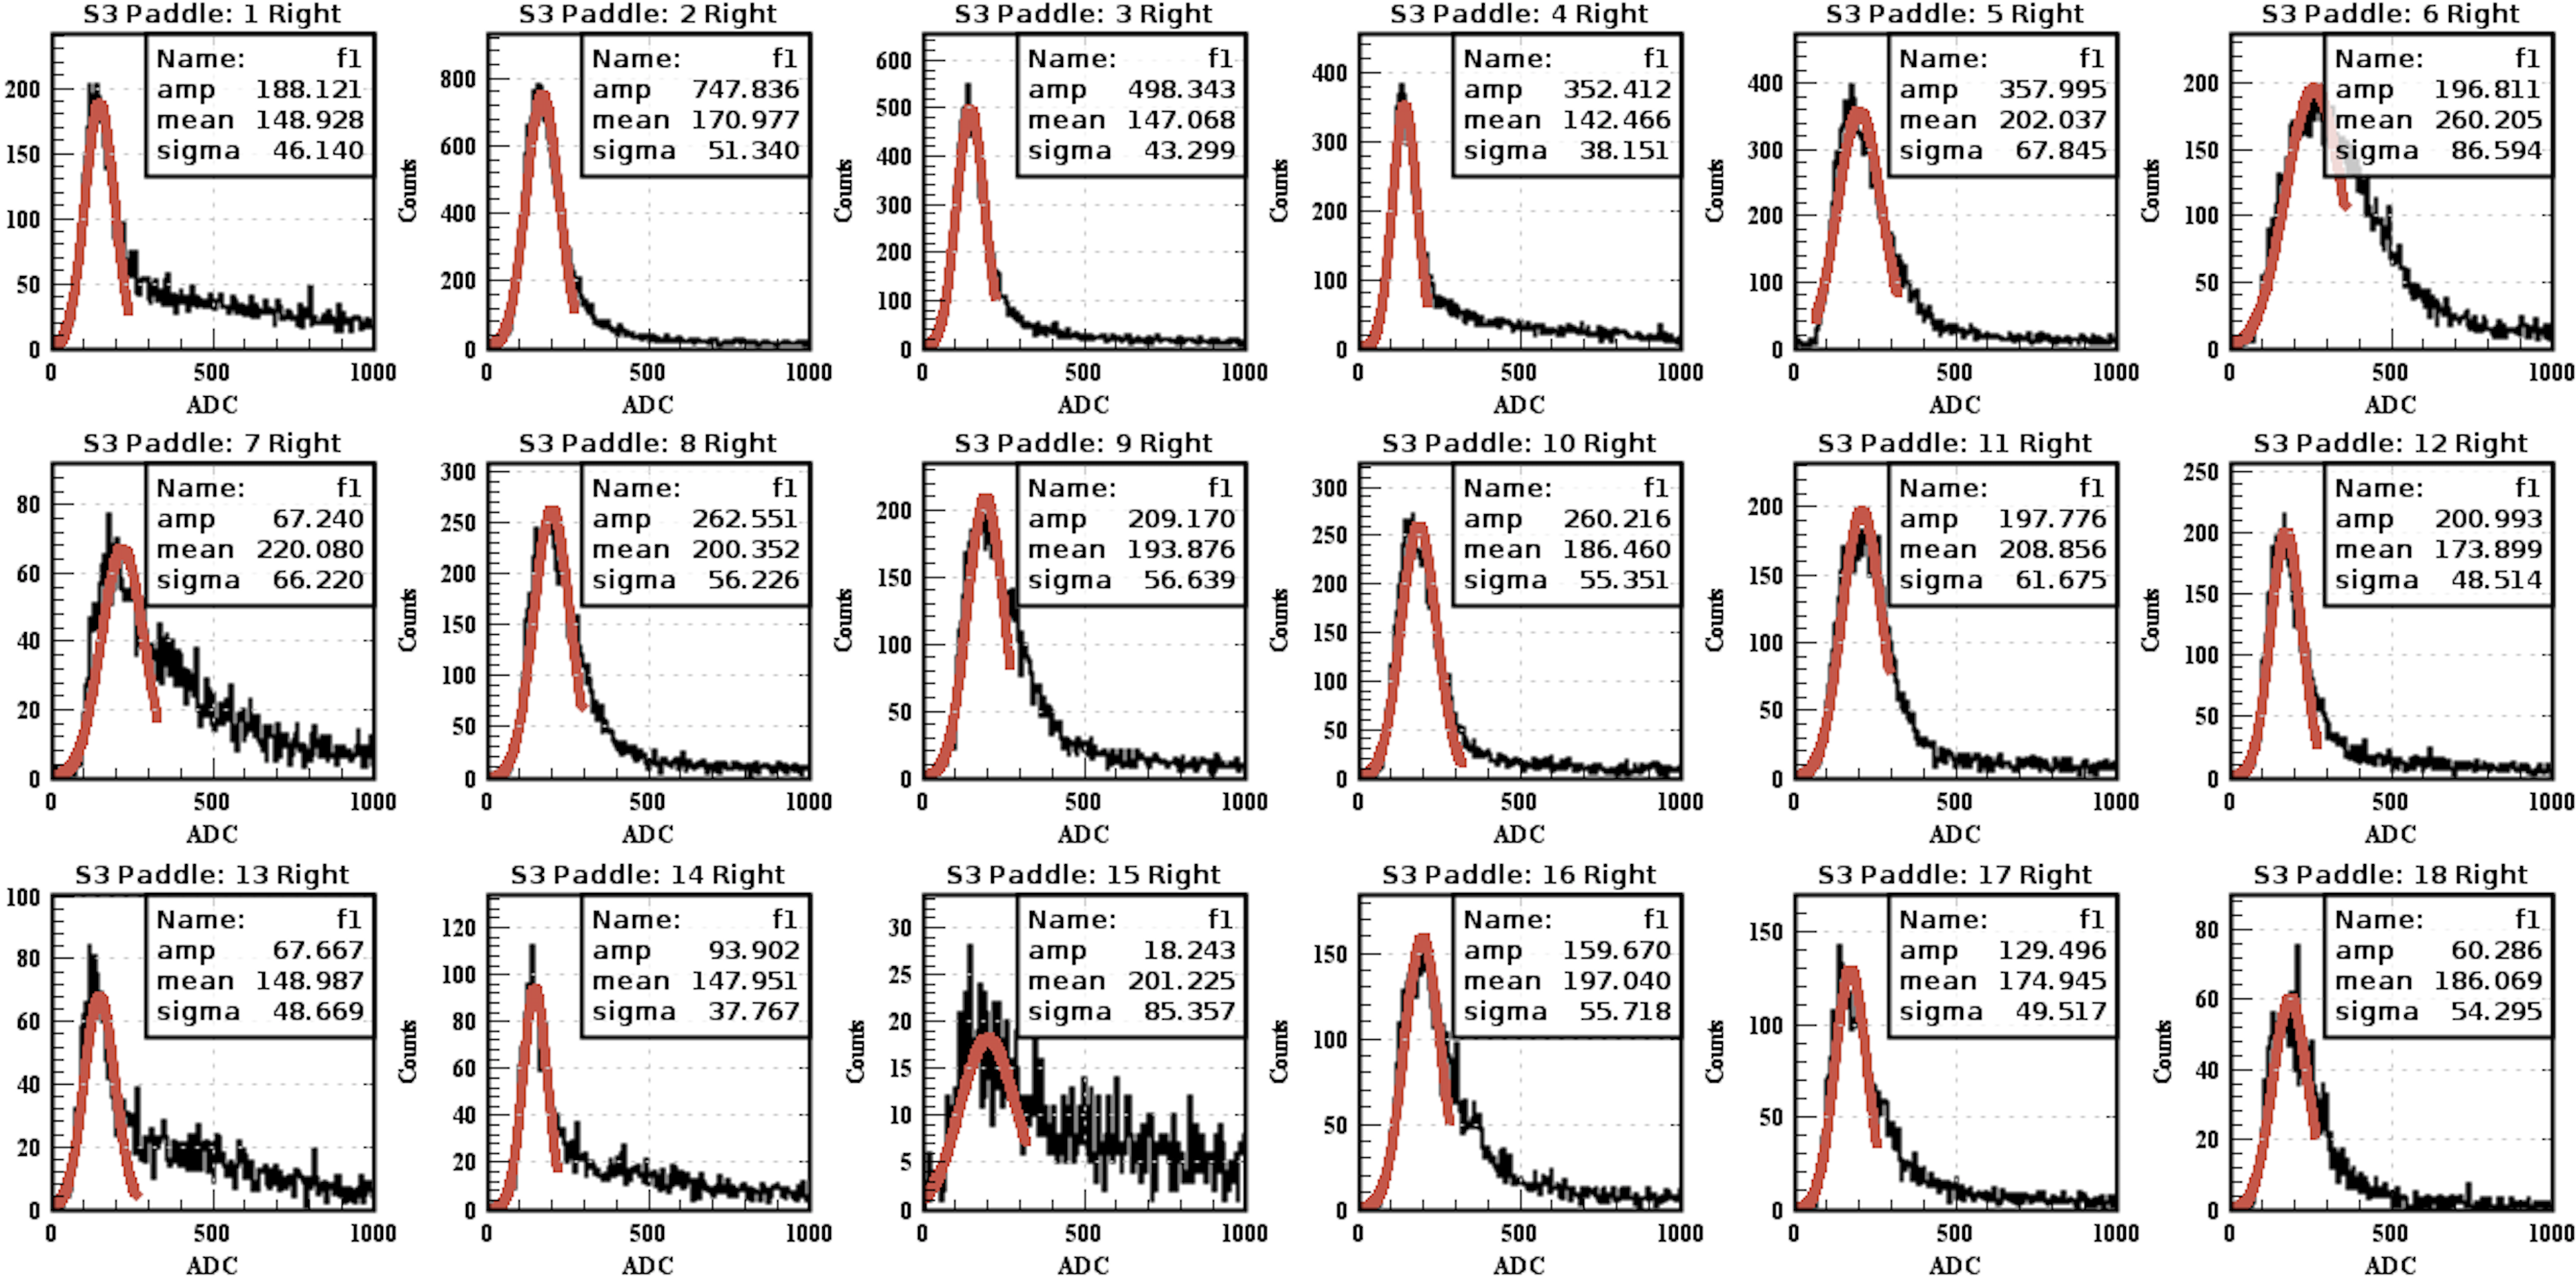
\includegraphics[width=1.99\columnwidth,keepaspectratio]{img/spe.png}
	\caption{The LTCC sector 3 right side ADC spectra. Data is from the first production run. The SPE peak positions are fitted and the mean $ADC_M$
            parameters are recorded in the calibration database. The reconstructed number of photo-electrons for the digitized ADC value is then ADC / $ADC_M$.}
	\label{fig:speCalibration}
\end{figure*}

This was accomplished by using normal the experiment production dataset.
A random trigger was saved in the data-stream using a pre-scale factor of 100.
This data subset has the LTCC events with PMT noise above the FADC trigger, containing the Single Photo-electron signal (SPE).

The spectra (see for \F{speCalibration} for typical histograms) were fitted to identify the SPE peak positions.
At the beginning of each experiment the PMT high voltage were modified to align the peak positions
to a particular ADC value of $ADC_M = 200$. An example of gain matching is shown in \F{gainMatching}.


\begin{figure}
	\centering
	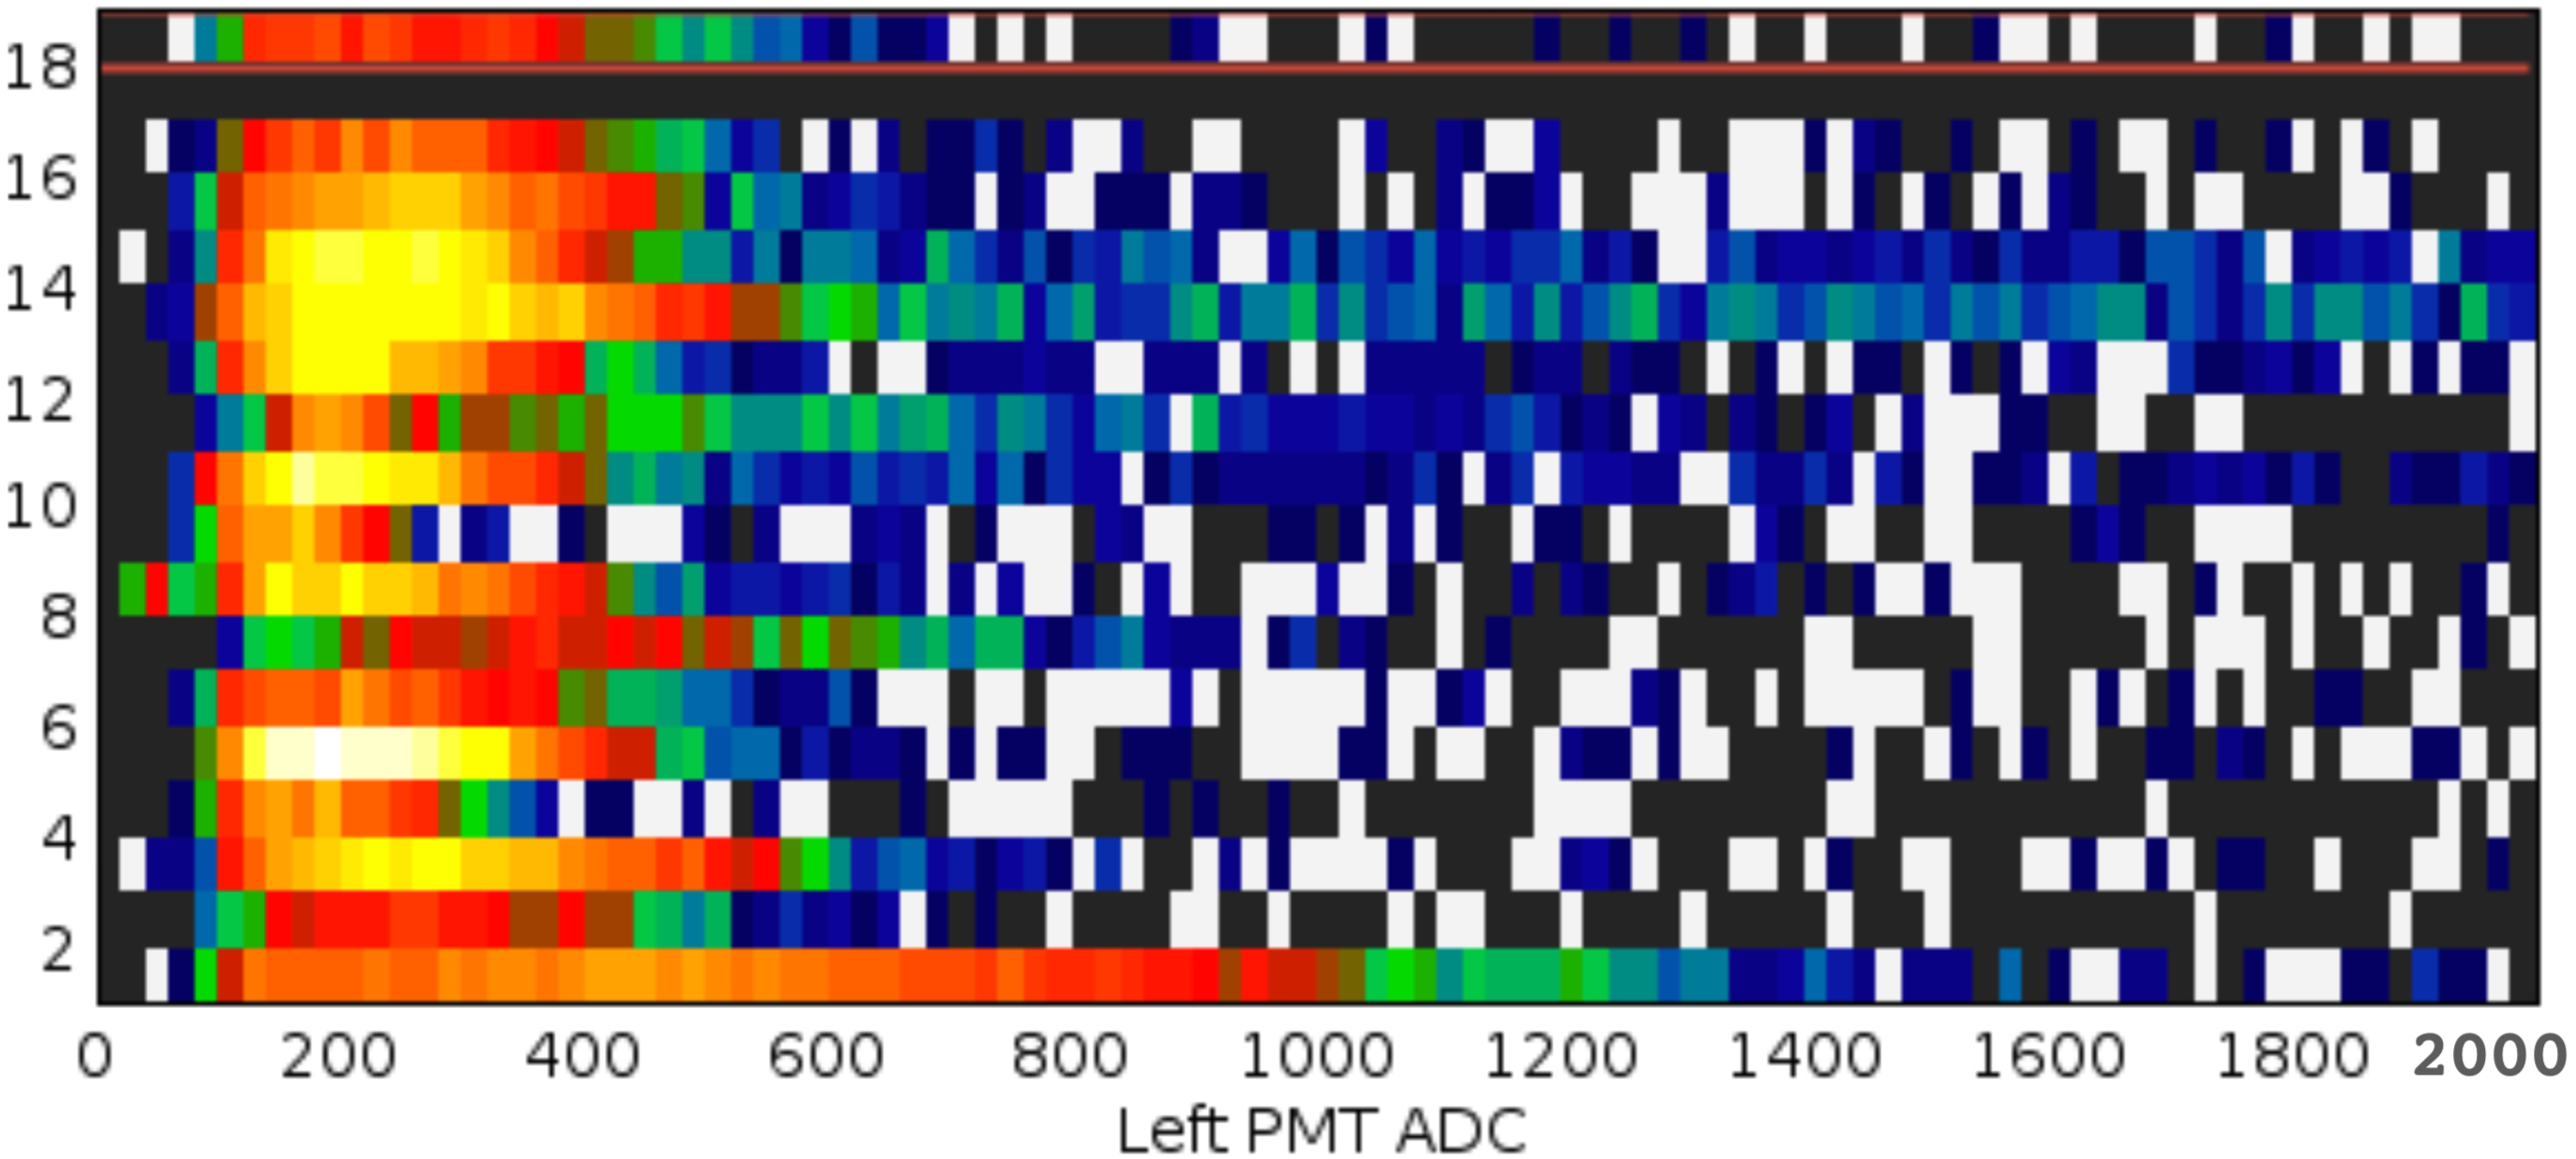
\includegraphics[width=0.95\columnwidth,keepaspectratio]{img/gainMatchingBefore.png}
	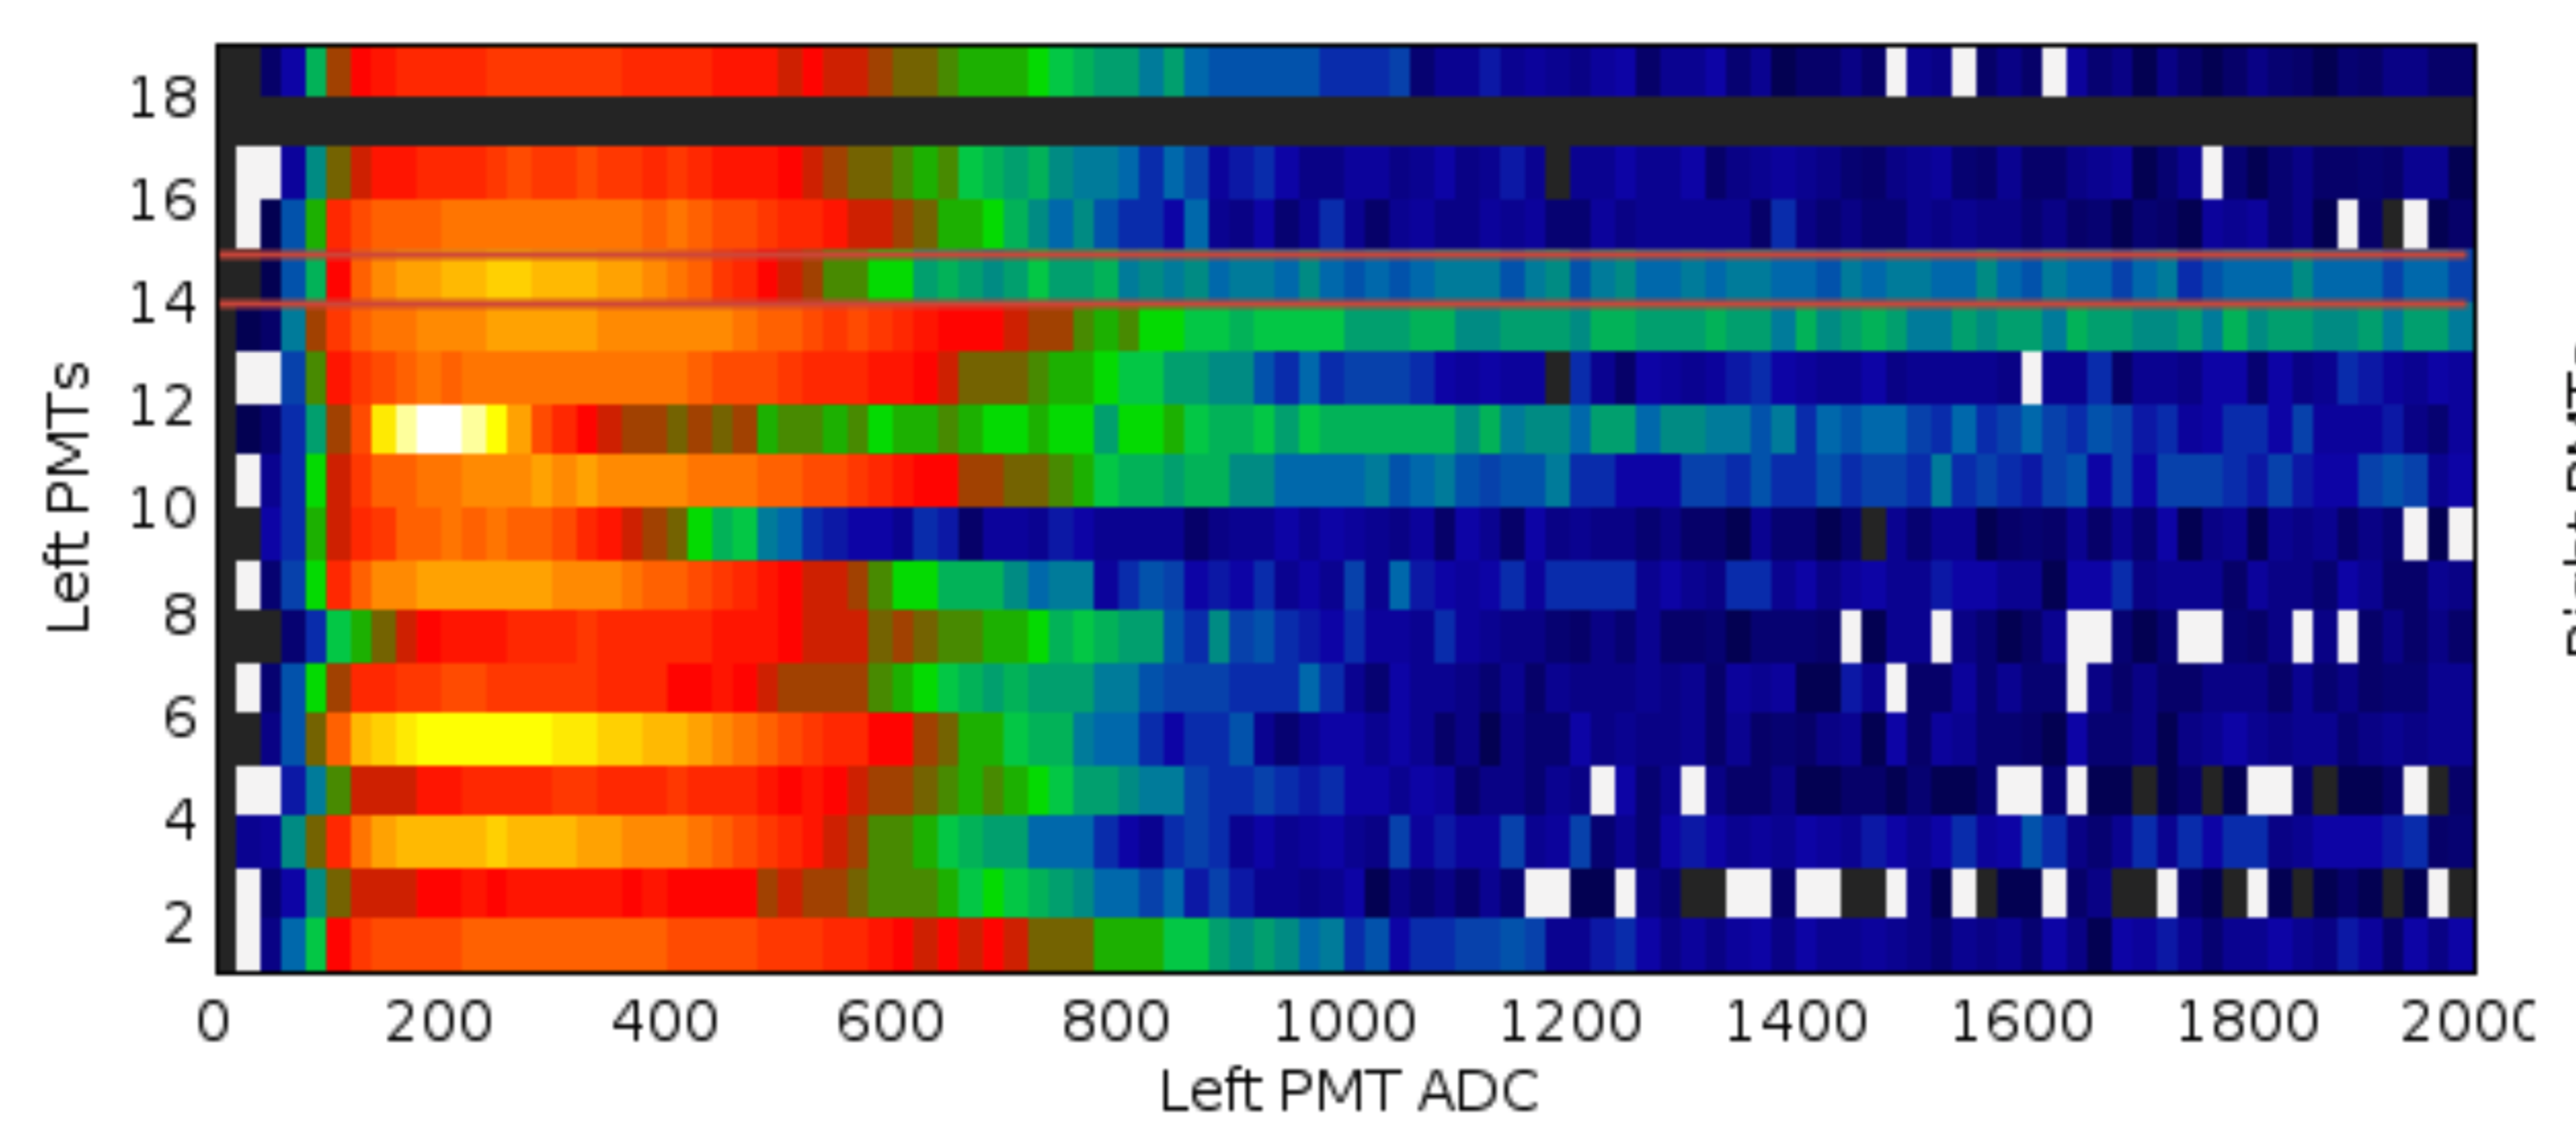
\includegraphics[width=0.95\columnwidth,keepaspectratio]{img/gainMatchingAfter.png}
\caption{The LTCC sector 3 left side PMT occupancies for each of the PMT as a function of channel. Data is from the first production run. Top: before gain matching
		   several channels do not show a SPE peak position at  $ADC_M = 200$. Bottom: after gain matching the PMT responses are more aligned.}
	\label{fig:gainMatching}
\end{figure}

During analysis of physics events, the reconstructed number of photo-electrons for the digitized ADC value calculated to be ADC / $ADC_M$.

It was found that the gains of several of the phototubes drifted with time, so the calibration procedure was repeated every week to ensure that
the values of $ADC_M$ reflects the latest gains and that these variation do not affect the LTCC response.



